\documentclass[11pt]{article}
\usepackage[margin=1in]{geometry}
\usepackage{graphicx}
\usepackage{booktabs}
\usepackage{amsmath}
\usepackage{amssymb}
\usepackage{xcolor}
\usepackage[hidelinks]{hyperref}
\usepackage{caption}
\captionsetup{font=small}

\title{\vspace{-2.5em}Characterisation of the sparks (full-detector discharges)
for detector~3\\\large (June cosmic bench --- \texttt{g\_det3\_wknd})}
\author{MX17 cosmic-bench QA}
\date{\today}

\begin{document}
\maketitle
\vspace{-1.5em}

\section{Setup}
A \textbf{spark} is an event in which the det3 readout fires more than
\textbf{50 strips} at once (summed over both planes) --- a full-detector discharge,
the same cut used to veto sparks in the efficiency breakdown. Run
\texttt{mx17\_det3\_p2\_det1\_overnight\_6-27-26 / long\_run\_p2} (headline det3):
6.9~h, 90\,914 detector-firing events, \textbf{8\,301 sparks} (9.1\,\% of firing
events, mean rate 0.33~Hz). Each spark hit carries a strip position (X$=$FEU7,
Y$=$FEU8), a time within the readout window, and an amplitude; each event carries a
timestamp and, where M3 reconstructs a clean single track, a ray projected onto the
det3 plane in the aligned frame (same geometry as the efficiency analysis). We answer
four questions.

\section{Result in one paragraph}
Sparks are \textbf{Poisson-random in time} (flat rate, no HV-recovery bursts) but
\textbf{not random with respect to the muon}: conditioning on a clean single muon, a
track that \emph{crosses} the detector sparks at $4.9\,\%$ versus only $1.2\,\%$ when it
clearly \emph{misses} --- a \textbf{4$\times$ enhancement}, so most in-detector sparks
are muon-induced on top of a $\sim$1.2\,\% spontaneous baseline. In detector coordinates
they are \textbf{localised}: strip occupancy peaks sharply at the plane \textbf{edges}
(plus a few hot strips), while the discharge centroid sits centrally. Temporally the
discharge is \textbf{neither a single flash nor a propagating ``walk''}: strips across a
$\sim$200~mm region fire over a spread $\sim$250~ns window (tail to $\sim$1~\textmu s)
with no position--time correlation.

\section{Q1 --- Are sparks random in time?  Yes (Poisson)}
The spark rate is flat at $0.33$~Hz across the entire 6.9~h run
(Fig.~\ref{fig:time}a): no bursts, no drift, so this is \emph{not} an HV-instability /
recovery-oscillation phenomenon. Inter-spark intervals follow a pure exponential over
three decades (Fig.~\ref{fig:time}b) and the sparks-per-10-min counts have
$\mathrm{std}=14=\sqrt{\mathrm{mean}}$ (Fig.~\ref{fig:time}c) --- textbook Poisson.
\emph{Caveat:} Poisson timing is expected for \emph{both} muon-induced and spontaneous
sparks (muons themselves arrive Poisson), so time-randomness alone does not settle
causation --- that is what Q2 is for.

\begin{figure}[h]\centering
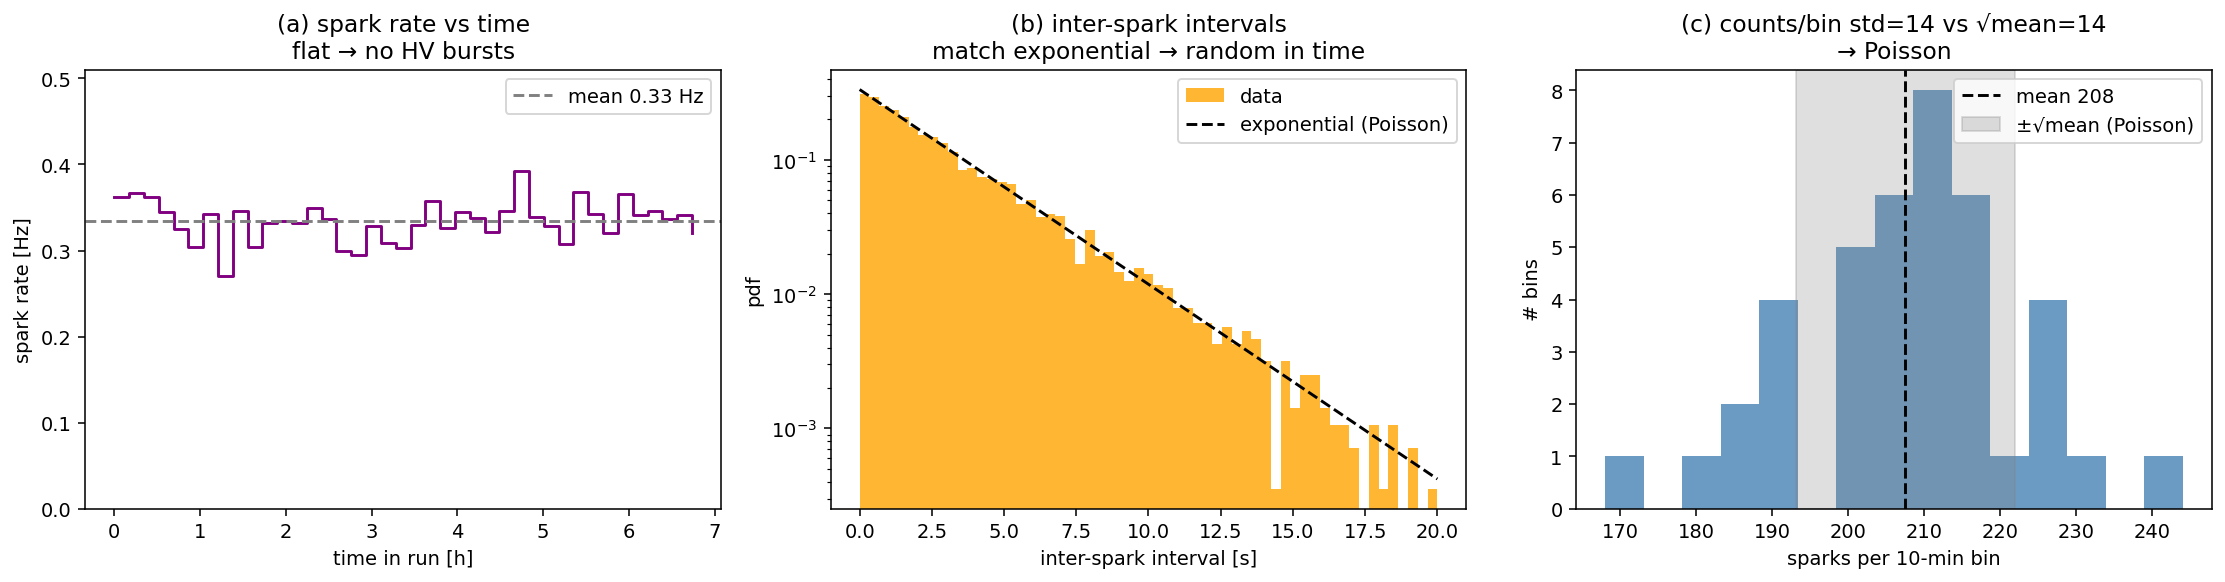
\includegraphics[width=\textwidth]{fig_time.png}
\caption{\textbf{Time.} (a) spark rate vs time in run; (b) inter-spark interval pdf with
the exponential expectation; (c) counts per 10-min bin vs the Poisson $\pm\sqrt{\text{mean}}$
band. Sparks are random in time with a stable rate.}
\label{fig:time}
\end{figure}

\section{Q2 --- Muon-induced or random?  Muon-dominated}
This is the decisive test (Fig.~\ref{fig:muon}a). Taking only events with a clean single
M3 muon and asking whether that muon's projection lands on the detector:
%
\begin{table}[h]\centering\small
\begin{tabular}{lrrr}
\toprule
muon geometry (clean single M3 track) & $N$ & sparks & spark rate\\
\midrule
crosses detector (ray in active box)        & 52\,995 & 2\,600 & \textbf{4.91\,\%}\\
at edge ($<$30~mm outside box)              & 9\,824  & 557    & 5.67\,\%\\
clearly misses ($>$30~mm outside box)       & 11\,858 & 141    & \textbf{1.19\,\%}\\
\midrule
(no clean M3 track --- see below)           & 36\,609 & 5\,003 & 13.67\,\%\\
\bottomrule
\end{tabular}
\end{table}
%
A muon that traverses the gas raises the spark probability \textbf{4.1$\times$} over one
that misses. So $\sim$75\,\% of in-detector sparks are \textbf{muon-induced} (the crossing
muon's primary ionisation seeds the discharge) and $\sim$25\,\% ($\approx$1.2\,\%
absolute) are a \textbf{spontaneous baseline} present even with no muon in the gas. In M3
coordinates the sparking muons are otherwise unremarkable --- roughly uniformly spread
over the acceptance (Fig.~\ref{fig:muon}b), i.e.\ no special beam/telescope location.

\paragraph{The ``no clean track'' population (a readout confound).}
$60\,\%$ of all sparks fall in events where M3 finds \emph{no} clean track, versus a
$33\,\%$ baseline --- sparks are $2\times$ over-represented there, and those sparks are
the \emph{same size} as the tracked ones (median 91 vs 95 strips). The most likely
reading is that a large discharge injects common-mode noise into the \emph{shared} DAQ
and spoils M3 track reconstruction for that event (or that both are triggered by a messy
multi-particle event). Either way it is a selection/cross-talk artefact, not evidence of
a large muon-independent spark source, so the clean $4.9\,\%$ vs $1.2\,\%$ comparison
above is restricted to good-track events. \emph{This DAQ cross-talk is itself worth a
follow-up.}

\begin{figure}[h]\centering
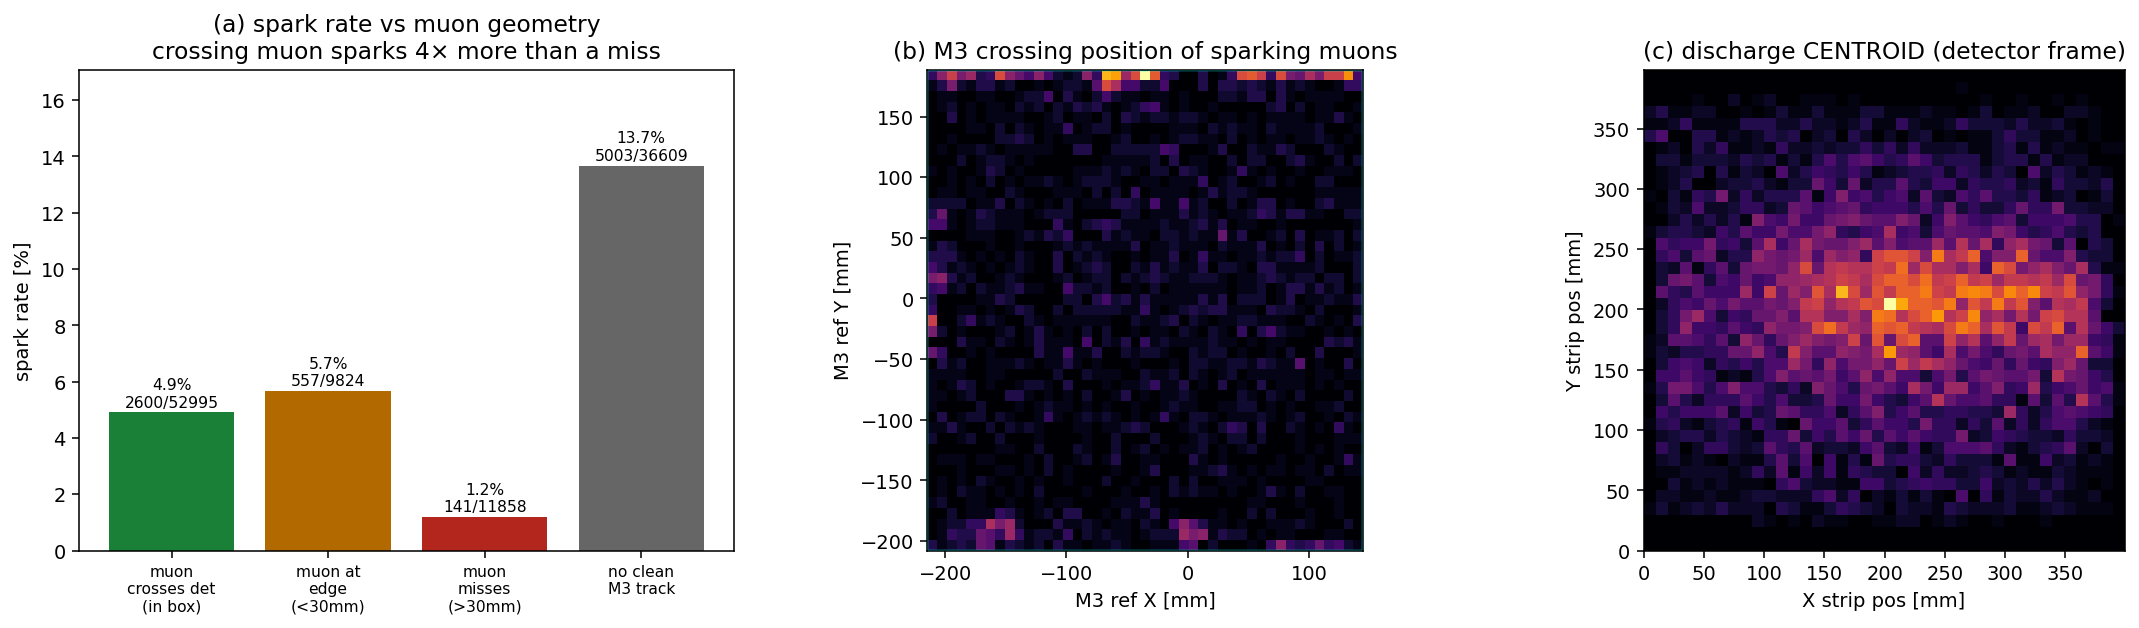
\includegraphics[width=\textwidth]{fig_muon.png}
\caption{\textbf{Muon dependence.} (a) spark rate split by where the muon projects ---
crossing muons spark $4\times$ more than missing ones; (b) M3 crossing positions of
sparking muons (roughly uniform); (c) discharge centroid in the detector frame
(central).}
\label{fig:muon}
\end{figure}

\section{Q3 --- Are there particular places that spark?  Yes: the edges}
Strip occupancy in sparks is strongly non-uniform (Fig.~\ref{fig:places}a,b). Both planes
show large peaks at the detector \textbf{edges} ($0$ and $\sim$$399$~mm; strongest at
high-$X$ and low-$Y$), where field lines concentrate at the active-area boundary --- edge
strips participate in a large fraction of all sparks. On top of the edge structure the
$Y$ plane (FEU8) shows a handful of narrow spikes at fixed positions --- individual
\textbf{hot strips} that fire far above average. Yet the discharge \emph{centroid} sits
centrally (Fig.~\ref{fig:muon}c): a typical spark ignites over a $\sim$200~mm span
(median $X$ span 204~mm, $Y$ span 235~mm of the 399~mm plane) --- roughly half the
detector, not a point and not the whole plane --- with the edges over-weighted. The
$Y$/FEU8 plane discharges harder than $X$ (median 53 vs 40 strips; Fig.~\ref{fig:places}c),
consistent with the FEU8 saturation band seen in the reco\_far study. Only $10\,\%$ of
spark hits actually saturate the ADC, so these are genuine spread discharges, not just
electronic rail-outs.

\begin{figure}[h]\centering
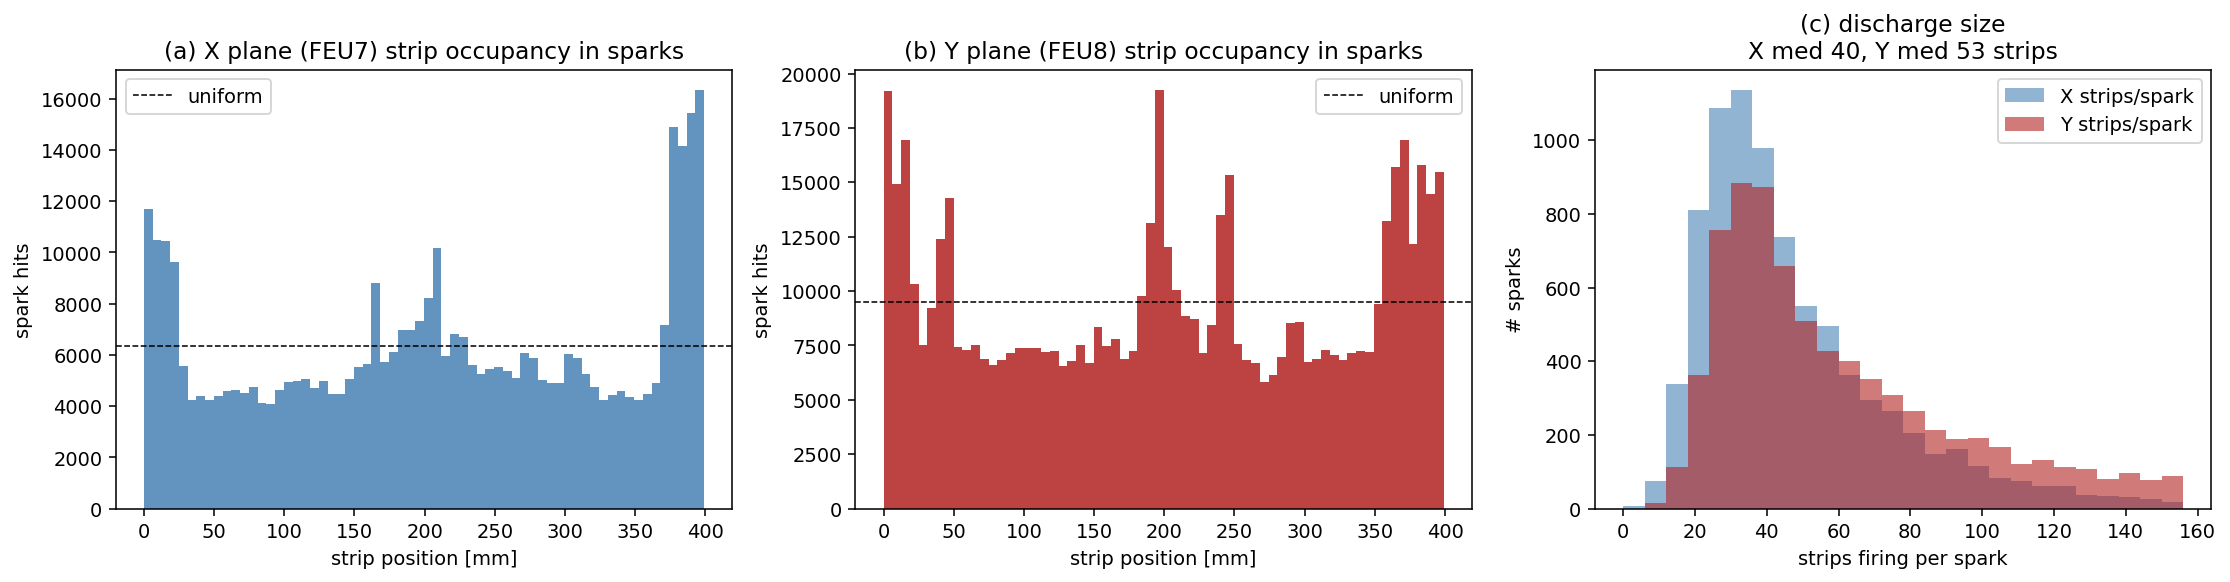
\includegraphics[width=\textwidth]{fig_places.png}
\caption{\textbf{Where.} (a,b) strip occupancy in sparks for the X and Y planes vs a
uniform baseline --- edge peaks (both planes) and fixed hot strips (Y); (c) strips firing
per spark --- Y discharges are larger than X.}
\label{fig:places}
\end{figure}

\section{Q4 --- All strips at once, or does the discharge ``walk''?  Neither}
The discharge is \emph{not} a single simultaneous flash: only $1.2\,\%$ of sparks have all
their hits within 100~ns; the per-spark hit-time spread is $\sigma\approx253$~ns median
(tail beyond 500~ns), somewhat broader than a normal drift cluster ($193$~ns,
Fig.~\ref{fig:walk}a). But it does \emph{not} propagate spatially either: the per-spark
position--time correlation is $|r|\approx0.12$ (only $3\,\%$ exceed $0.5$), and the
spark-centred $\Delta\text{position}$--$\Delta\text{time}$ map (Fig.~\ref{fig:walk}b) is a
clean \textbf{cross with no tilt} --- a horizontal arm (strips across the whole span
firing near-simultaneously) plus a vertical arm (the core keeps firing over
$\pm$hundreds of ns), and no diagonal that a moving front would produce. Example events
(Fig.~\ref{fig:walk}c) show strips lighting up across the full $0$--$400$~mm range at
scattered times. \textbf{Picture:} a spatially-extended discharge that fires a broad
region in a near-synchronous burst and then rings/afterpulses for up to $\sim$1~\textmu s,
with timing independent of position --- not a wave sweeping across the strips.

\begin{figure}[h]\centering
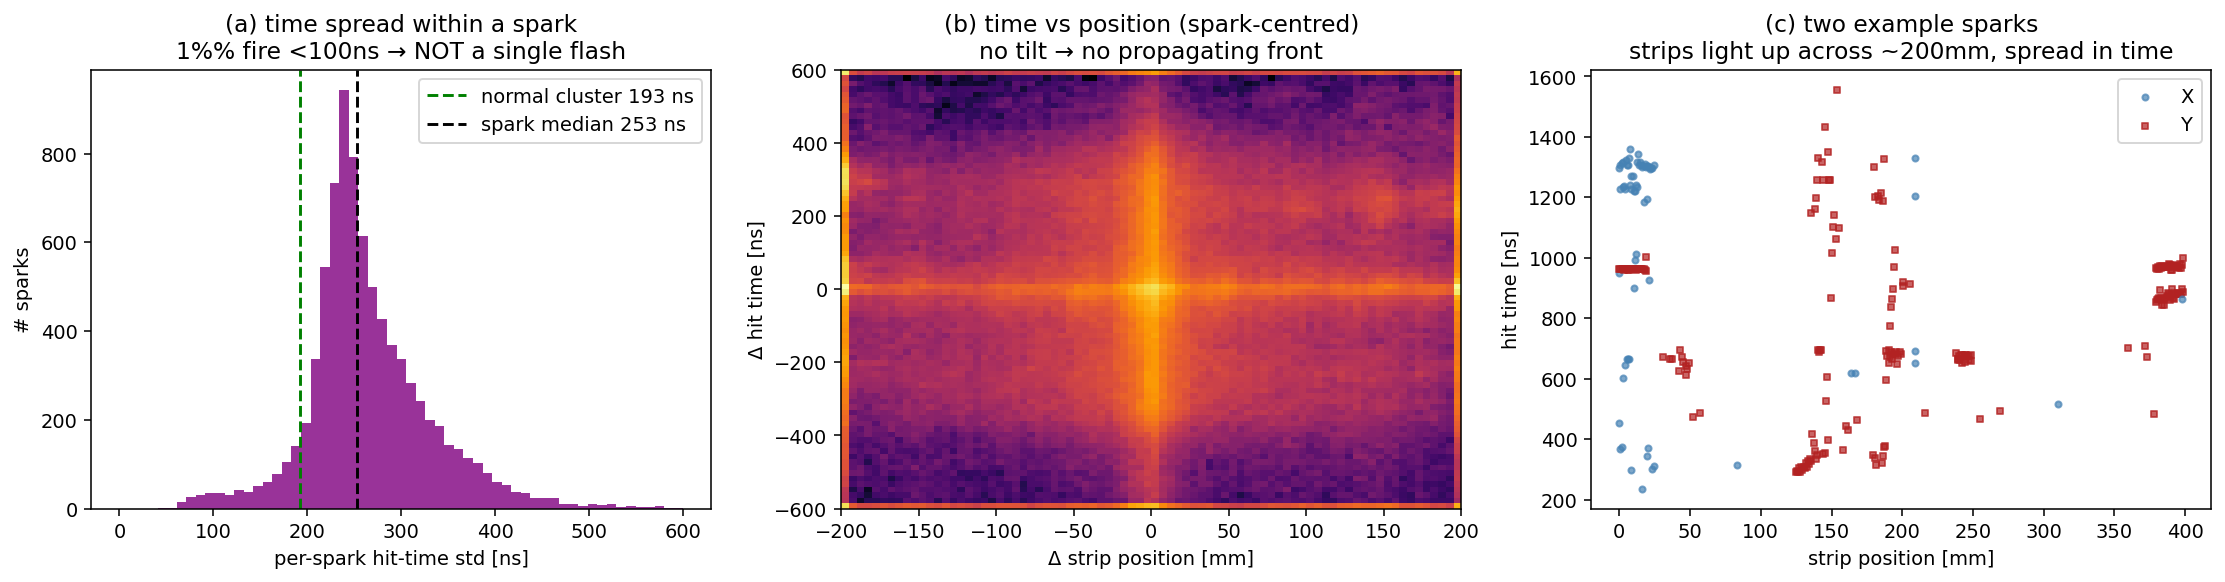
\includegraphics[width=\textwidth]{fig_walk.png}
\caption{\textbf{Time structure.} (a) per-spark hit-time spread vs a normal cluster;
(b) spark-centred time vs position (no tilt $\Rightarrow$ no propagating front);
(c) two example sparks --- strips across $\sim$400~mm, spread in time, no position ramp.}
\label{fig:walk}
\end{figure}

\section{Summary and follow-ups}
\begin{itemize}\setlength\itemsep{0.15em}
  \item \textbf{Time:} Poisson-random, stable $0.33$~Hz --- not HV bursting.
  \item \textbf{Cause:} predominantly \textbf{muon-induced} --- a crossing muon sparks
        $4\times$ more than a missing one ($4.9\,\%$ vs $1.2\,\%$) --- on a $\sim$1.2\,\%
        spontaneous floor. Lowering the resist HV reduces the \emph{rate} (fewer avalanches
        reach breakdown) but cannot remove the muon-seeded component entirely.
  \item \textbf{Place:} \textbf{edge-dominated} occupancy plus fixed hot strips (Y/FEU8);
        discharges span $\sim$half the plane, centred centrally; Y sparks harder than X.
  \item \textbf{Structure:} a spatially-extended, temporally-spread ($\sim$250~ns, tail to
        $\sim$1~\textmu s) discharge with afterpulsing --- no propagating ``walk''.
  \item \textbf{Follow-ups:} (1) inspect the edge / guard-ring field and the Y/FEU8 hot
        strips (mask or lower gain); (2) confirm and mitigate the \textbf{DAQ common-mode
        cross-talk} by which a det3 spark spoils M3 tracking (60\,\% of sparks lose the M3
        track); (3) an offline spark tag (multiplicity $+$ the $\sim$1~\textmu s duration
        signature) would clean the reco\_far tail (companion note
        \texttt{det3\_recofar\_analysis}).
\end{itemize}

\vspace{0.4em}
\footnotesize\noindent\textit{Reproduce:} \texttt{extract\_sparks.py} then
\texttt{make\_plots.py}; numbers in \texttt{spark\_meta.json}. Spark cut ($>$50 strips)
and alignment match \texttt{09\_efficiency\_breakdown.py}.

\end{document}
